% % Full page illustration
% \begin{figure}[!hbtp]
%     \centering
%     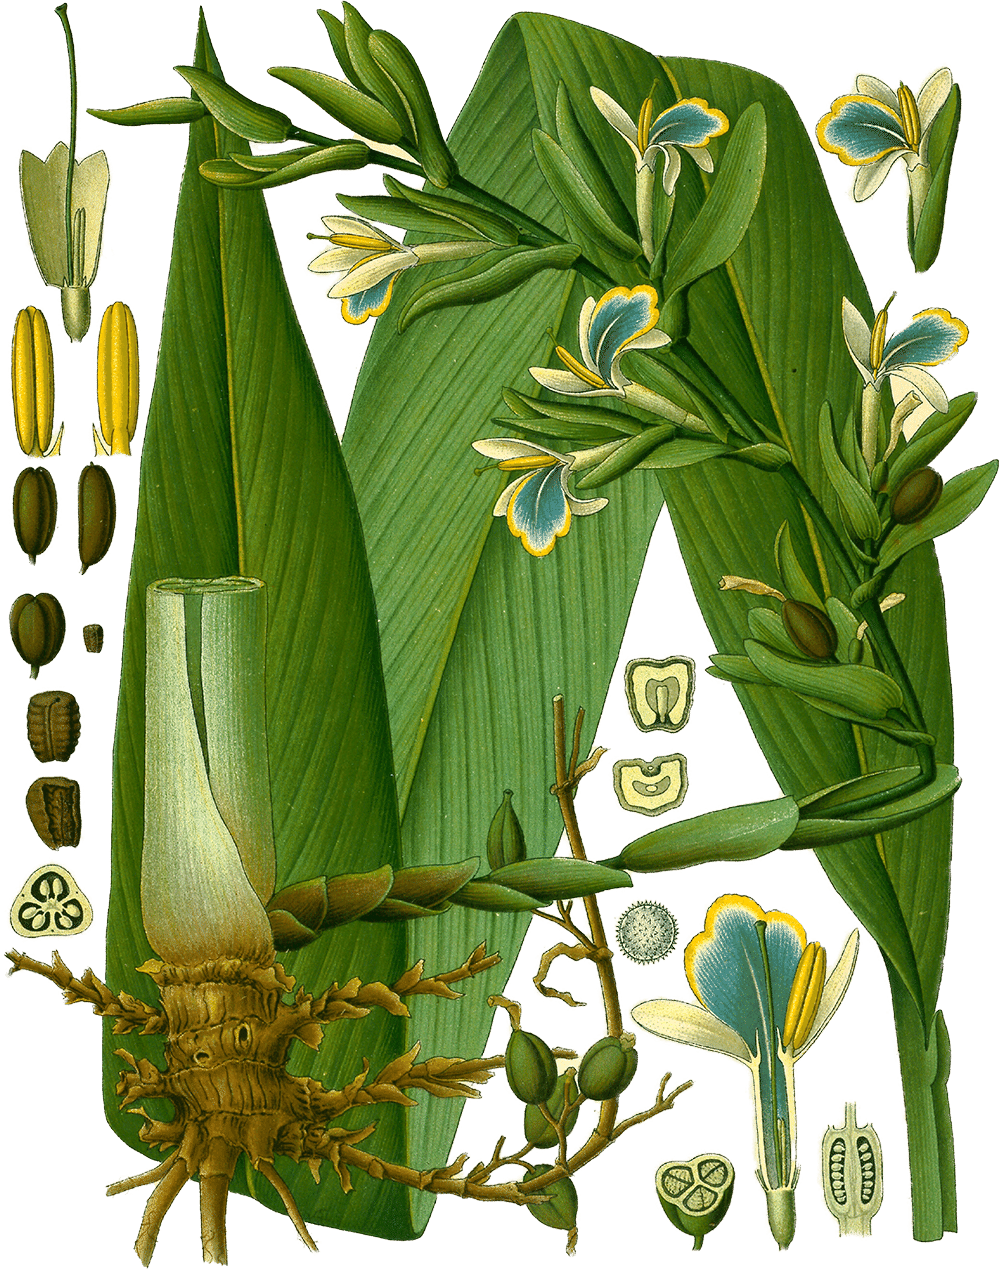
\includegraphics[width=\textwidth]{imgs/kohler/cardamom_kohler_min.png}
%     \caption{\taxonn{Elettaria cardamomum}{(L.) Maton} (syn. \taxonn{Amomum cardamomum}{L.}), the cardamom plant in Köhler's Medicinal Plants \pvolcite[]{2}[186]{kohler_kohlers_1887}.}
%     \label{fig:kohler_cardamom}
% \end{figure}



\section{Cardamom}
\label{sec:cardamom}\label{sec:black_cardamom}

\begin{spice}\label{spice:cardamom}
\textsc{Cardamom} \hfill \href{https://powo.science.kew.org/taxon/796556-1}{POWO} \\
\textbf{English:} \textit{cardamom}. 
\textbf{Arabic:} {\arabicfont{هال}} \textit{hāl}; {هيل} \textit{hayl}. 
\textbf{Chinese:} {\tradchinesefont{豆蔻}} \textit{dòukòu} [bean-cardamom]; 荳蔻. 
\textbf{Hungarian:} \textit{kardamom}.  \\
\noindent{\color{black}\rule[0.5ex]{\linewidth}{.5pt}}
\begin{tabular}{@{}p{0.25\linewidth}@{}p{0.75\linewidth}@{}}
Plant species: & \taxonn{Elettaria cardamomum}{(L.) Maton} (syn. \taxonn{Amomum cardamomum}{L.}) \\
Family: & \textit{Zingiberaceae} \\
part used: & fruit (seed pods, capsules) \\
Region of origin: & India \\
Cultivated in: & Guatemala; India; Sri Lanka; Tanzania; Papua New Guinea \\
Color: & green seed pods, brown seeds \\
\end{tabular}
\end{spice}

\begin{figure}[!ht]
	\vspace{-2ex}
	\centering
	\subfloat{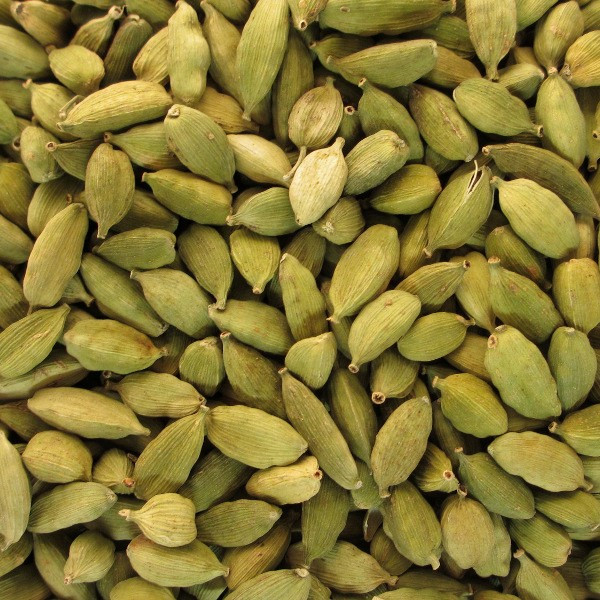
\includegraphics[width=0.3\linewidth]{imgs/spices/cardamom-1.jpg}}
	\hfill
	\subfloat{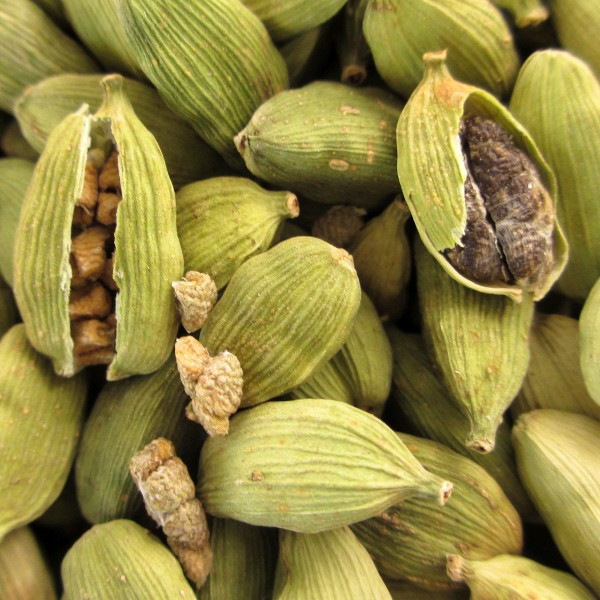
\includegraphics[width=0.3\linewidth]{imgs/spices/cardamom-2.jpg}}
	\hfill
	\subfloat{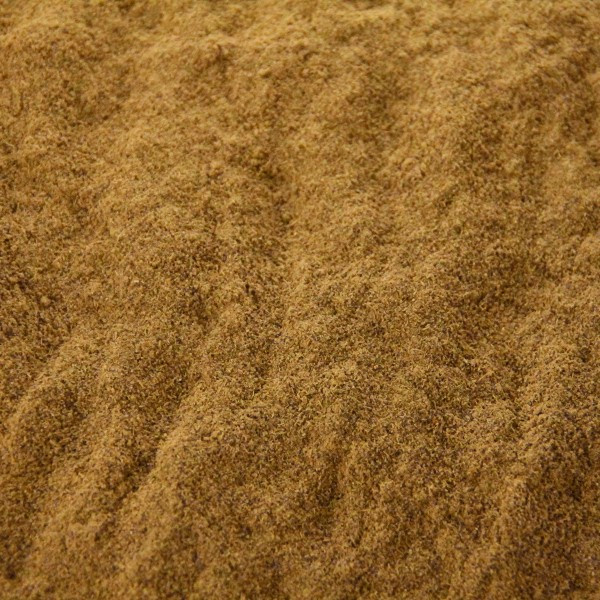
\includegraphics[width=0.3\linewidth]{imgs/spices/cardamom-3.jpg}}
	\caption[True cardamoms]{Cardamom fruits cured, and powdered (\textit{Elettaria cardamomum}). Credit: Aromatiques.}
	\label{fig:cardamom_imgs}
\end{figure}

Cardamoms are the dried, ripe fruits of the cardamom plant \textit{Elettaria cardamomum}. These fruits are sometimes called seeds, but they are in fact the seed pods, ``three-valved capsules'' \autocite[132]{van_wyk_culinary_2014}, containing several brown-colored small seeds, as it can be seen in \cref{fig:cardamom_imgs}. The cardamom of commerce is widely used in Asia as medicine and spice, and is valued for its unique, minty and eucalyptus-like flavor. It is most prevalent in Indian cooking, but also known from the Arabic coffee tradition where it is sometimes added to the beverage. Indian restaurants often place a bowl of cardamoms at the entrance, so customers can take one as a masticatory on their way out, and chew on the refreshing capsules as they were nature's breath mints. Native to the same region as the mighty black pepper in India, cardamom is sometimes referred to as the ``queen of spices'' \autocite[1]{ravindran_cardamom_2002}. Cardamom was imported to Europe since the Roman era, and it is still used in meat dishes, sausages, Swedish meatballs, Danish pastries, ice-cream and liqueurs \autocite[326]{mabberley_mabberleys_2017}. It is the third most expensive spice of our times, after saffron and vanilla \autocite{business_insider_why_2021}.

Although \textit{cardamom} usually refers to the fruits of \textit{E. cardamom} from India---also sometimes known as green cardamom and true cardamom---there are numerous other cardamoms, similarly segmented capsule-like fruits used as spices and medicine in South, Southeast, and East Asia, and even in Africa. Many of these belong to the \textit{Amomum} genus of the ginger family (\textit{Zingiberaceae}), such as the black cardamom from the Himalayas (\textit{Amomum subulatum}), and the round cardamom from Java (\textit{Amomum compactum}). See them in detail below in \cref{sec:crowd_of_cardamoms}.

% Aromatiques:

% Elettaria cardamomum

% Green cardamom, "queen of spices" in India, is indeed one of the most original and enchanting ones. From the zingiberaceae family, this beautiful plant is grown mainly in India, Sri Lanka or Guatemala. Naturally green and perfumed, the pods are only dried. Their powerful fragrance is very aromatic, hot and peppery but also camphor and menthol, durable and slightly numbing, making it a sovereign spice. We sometimes find white cardamom, these are the same pods, originally green, discoloured with sulfur and soap baths for an aesthetic purpose, they are less aromatic than green ones. Cardamom is used, either peeled: by opening the fruit to release the small black-grey seeds to be mortared (10-20 per pod); or whole in infusion in simmered dishes or cooking water.

% Traditionally used in Indian cuisine, green pods are an essential element of many dishes such as curry, dhal, rice. Cardamom powder is also present in classic mixtures such as masal garam or some curries. In sweet and savoury we find it in chutneys recipes. In Europe, cardamom is associated in salted with charcuterie or fish.

% Desserts are also greatly improved by cardamom: fruit salads, cakes, lassis, ice cream, gingerbread. It goes perfectly with chocolate: mousse, fondant, ice cream...

% Green cardamom is used in several traditional drinks in different parts of the world: it is added to coffee in the Middle East, mixed with other spices to prepare chaï masala in India, mulled wine in Europe or hypocras since the Middle Ages. It is also an ingredient of choice for flavoring punch and rhum arrangé.

% Chewing green cardamom seeds is very pleasant and refreshes the breath thanks to its fresh and minty aroma. It is also possible to neutralize the stubborn smell of garlic by this means.

% Cardamom has been recognized for millennia in Indian Ayurvedic medicine and Chinese medicine for its anti-acide, carminative, stomachic, appetizer and anti-nausea digestive properties.

% Amomum subulatum

% Also known as cardamom from China or Nepal, or fake cardamom, these large brown pods have a strong smoky scent and a very pronounced camphor taste. Smoked in wood fire, the coarse shell that contains the seeds concentrates essentially this smoky aroma, so we keep the whole pod, with its bark, to benefit the best in the kitchen. We only keep the seeds, possibly crushed in a mortar, if we want to highlight the camphor flavor

% Brown cardamom is mainly used as a spice in the preparation of Indian curry and other savory dishes from India that simmer for a long time. It is also associated with green cardamom in some recipes. To be added to chickpea, coral lentil or potato dishes to give a slightly raw and woody note.


% WIKI
%     True or green cardamom (or when bleached, white cardamom[12]) comes from the species Elettaria cardamomum and is distributed from India to Malaysia. What is often referred to as white cardamon is actually Siam cardamom, Amomum krervanh.[13]
%     Black cardamom, also known as brown, greater, large, longer, or Nepal cardamom, comes from species Amomum subulatum and is native to the eastern Himalayas and mostly cultivated in Eastern Nepal, Sikkim, and parts of Darjeeling district in West Bengal of India, and southern Bhutan.

% The two types of cardamom, καρδάμωμον and ἄμωμον, were distinguished in the fourth century BCE by Theophrastus. He reports that some people believed they came from Media, others from India.[14] 


% wiki:
% Amomum subulatum, also known as Black cardamom, hill cardamom,[1] Bengal cardamom,[1] greater cardamom,[1] Indian cardamom,[1] Nepal cardamom,[1] winged cardamom,[1] big cardamon,[2][3] or brown cardamom, is a perennial herbaceous plant in the family Zingiberaceae. Its seed pods have a strong, camphor-like flavour, with a smoky character derived from the method of drying. In Hindi it is called बड़ी इलाइची (baḍī ilāichī).
% Contents

%     1 Characteristics
%     2 Species
%     3 Medical production
%     4 See also
%     5 References

% Characteristics

% The pods are used as a spice, in a similar manner to the green Indian cardamom pods, but with a different flavour. Unlike green cardamom, this spice is rarely used in sweet dishes. Its smoky flavour and aroma derive from traditional methods of drying over open flames.
% Species

% At least two distinct species of black cardamom occur: Amomum subulatum (also known as Nepal cardamom) and Amomum tsao-ko. The pods of A. subulatum, used primarily in the cuisines of India and certain regional cuisines of Pakistan, are the smaller of the two, while the larger pods of A. tsao-ko (Chinese: wiktionary:草果; pinyin: cǎoguǒ; Vietnamese: thảo quả) are used in Vietnamese cuisine and Chinese cuisine, particularly that of Sichuan province.
% Medical production

% The largest producer of the black cardamom is Nepal, followed by India and Bhutan. In traditional Chinese medicine, black cardamom is used for stomach disorders and malaria.[dubious – discuss] In the traditional medicine of India, decoction of Amomum subulatum rhizomes is used in the therapy of jaundice.[4] 

\subsection{The Botany, Origins, and Cultivation of Cardamom}

The cardamom plant is a tall perennial herb from the ginger family (\textit{Zingiberaceae}) with pink white flowers that grow at the base of the stem in clusters \autocite[132]{van_wyk_culinary_2014}. \textit{Elettaria cardamomum} is indigenous to the Western Ghats region in South India, the same area that gave us black pepper and the center of its production and biodiversity \autocite[1]{ravindran_cardamom_2002}. Together with black pepper and ginger, it has been wild-harvested since time immemorial, and formed the livelihood of many from the beginnings of the ancient spice trade around the \nth{3} century \BC{}, until today \autocite[132]{van_wyk_culinary_2014}. Cardamom can only grow in a tropical climate, thriving in higher altitudes in the shade of trees, similarly to black pepper (which is a climbing vine) and thus modern cultivation does not differ much from traditional wild harvesting \autocite[132]{van_wyk_culinary_2014}. Cardamom is hand picked when ripe or near-ripe one by one---explaining its relatively high price---and then dried. It generally comes in light green, but one can also find them in white, which is a result of an extra step of steaming or bleaching before the drying process \autocite[132]{van_wyk_culinary_2014}. From the 1920s, Guatemala gradually became a major cardamom exporter, surpassing India in production. It is also grown in Tanzania and Papua New Guinea on a small scale.

\subsection{The History of Cardamom}

It is difficult to trace the history of cardamoms with certainty because of the confusion in nomenclature \autocite{cumo_encyclopedia_2013}. However, the cardamom described in \nth{4} century \BC{} in Indian Ayurvedic literature is probably the green or true cardamom of today, called \textit{el\={a}}\footcite[232]{monier-williams_sanskrit-english_1899} in Sanskrit. Cardamom was also described by Theophrastus in the \nth{4} century \BC{}. He reports that \textit{kardamomon} and \textit{amomon} (cardamom and black cardamom) come from Media, or according to some, from India---just like spikenard and most other spices \autocite[249]{theophrastus_enquiry_1916}. Pliny connects amomum to North India, which is quite a punctual source for black cardamom. Cardamom was known to Dioscorides and Hippocrates, who have both written on its health benefits, e.g.,aiding digestion. In Modern Greek, there is an informal way of saying `to strengthen, get strong': \gr{καρδαμώνω} \textit{kardamóno}\footnote{\url{https://www.greek-language.gr/greekLang/modern_greek/tools/lexica/triantafyllides/search.html?lq=\%CE\%BA\%CE\%B1\%CF\%81\%CE\%B4\%CE\%B1\%CE\%BC\%CF\%8E\%CE\%BD\%CF\%89\&dq=}} deriving from the name of the spice.

Medieval Arab doctors wrote about cardamom in similar ways, and the geographer al-Idrīsī described  ca. 1150 that it is brought to the port of Aden from Sindh, India and China, whereas in China, black cardamoms were important in the economy of the Song period (960–1279) \autocite[158-159]{prance_cultural_2005}. Green cardamom reached China from Southeast Asia, in Hong Kong it is consumed primarily by the Indians and the Portuguese. It is cultivated in Guangdong, Guangxi, and Yunnan, rather used in medicine than cooking \autocite[325-326]{hu_food_2005}. For more on cardamom's history, see \textcite[102-106]{dalby_dangerous_2000}.

% USES
% wyk
% culinary uses The delicious sweetish and pungent taste of cardamom has found its way into many different culinary traditions. In its native India, cardamom forms an important component of curries and curry powders. It is also widely used in rice, vegetable and meat dishes, as well as sweet desserts. The seeds are traditionally used to flavour Arabian coffee and black Turkish tea.3 In Europe and America, cardamom is well known as an essential ingredient of gingerbread and sweet pastries. Scandinavians (especially Swedes and Finns) are particularly fond of cardamom and large amounts are used in confectionery, desserts, stewed fruits, mulled wines, meat dishes and sausages.3 Ground cardamom is added to hamburger patties and meatloaf – one teaspoon per kg (2.2 lb.), while roughly bruised seeds are used in sausages as well as in breads, buns and brioches.3 Flavour compounDs The essential oil contains 1,8-cineole (eucalyptol) and α-terpinyl acetate as major compounds, but the typical aroma of cardamom is ascribed to trace amounts of unsaturated aliphatic aldehydes such as (E)-4-decenal.4 notes For Ethiopian cardamom (korarima), see Aframomum corrorima.

\subsection{A Crowd of Cardamoms: Identity and Confusion with Other Spices}
\label{sec:crowd_of_cardamoms}

% \begin{spice}\label{spice:black cardamom}
\textsc{Black cardamom} \hfill \href{https://powo.science.kew.org/taxon/urn:lsid:ipni.org:names:872166-1}{POWO} \\
\textbf{English:} \textit{black cardamom}; \textit{brown cardamom; greater cardamom; Indian cardamom; Nepal cardamom; Indian black cardamom; Bengal cardamom; big cardamom; hill cardamon; winged cardamom; fake cardamom; false cardamom; amomum*}. 
\textbf{Arabic:} {\arabicfont{قاقلة}} \textit{qāqulla}. 
\textbf{Chinese:} {\tc{香豆蔻}} \textit{xiāngdòukòu} [fragrant-cardamom]; \tc{嘎哥拉} \textit{gāgēlā}. 
\textbf{Hungarian:} \textit{fekete kardamom} [black cardamom].  \\
\noindent{\color{black}\rule[0.5ex]{\linewidth}{.5pt}}
\begin{tabular}{@{}p{0.25\linewidth}@{}p{0.75\linewidth}@{}}
Plant species: & \taxonn{Amomum subulatum}{Roxb.} \\
Family: & \textit{Zingiberaceae} \\
Plant part used: & fruit & seed \\
Region of origin: & Nepal to Central China \\
Cultivated in: & Himalayas \\
Color: & dark brown \\
\end{tabular}
\end{spice}

%picture of red cardamom and korarima?

\begin{figure}[!ht]
	\vspace{-2ex}
	\centering
	\subfloat[]{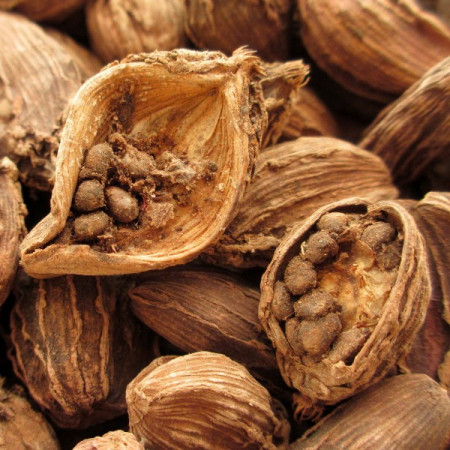
\includegraphics[width=0.3\linewidth]{imgs/spices/cardamom-black-1.jpg}}
    \hfill
	\subfloat[]{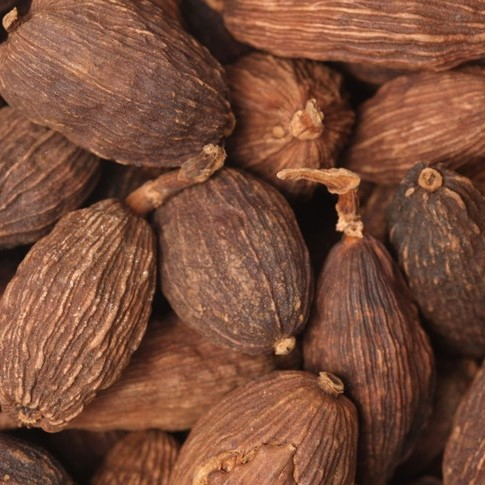
\includegraphics[width=0.3\linewidth]{imgs/spices/cardamom-chinese-1.jpg}}
    \hfill
	\subfloat[]{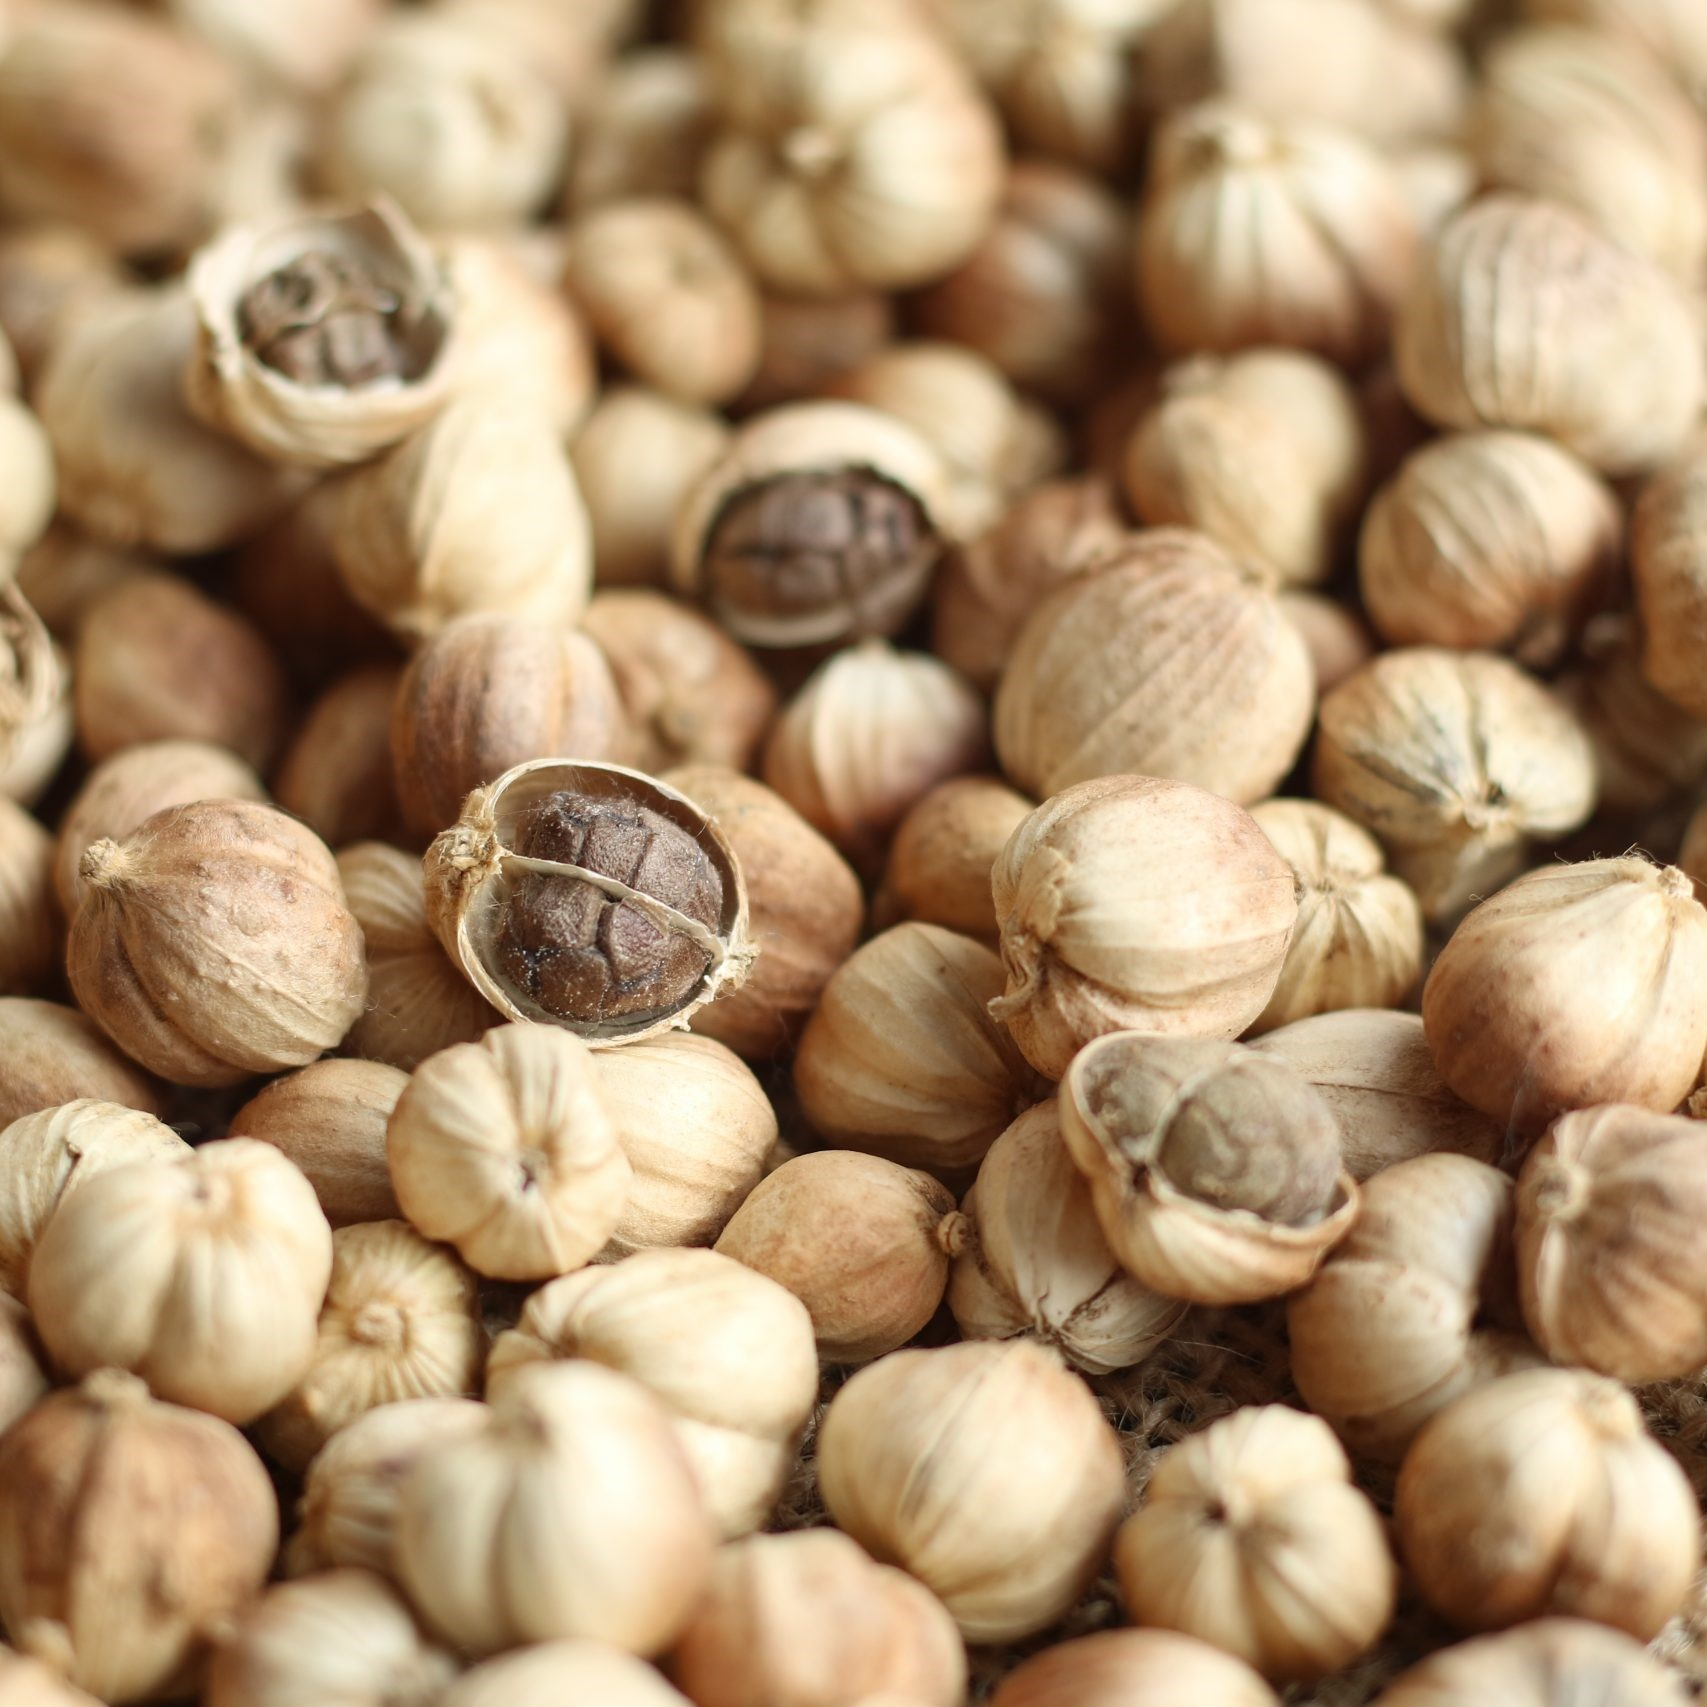
\includegraphics[width=0.3\linewidth]{imgs/spices/cardamom-white-1.jpg}}
	\caption[False cardamoms]{False cardamoms: (a) Black cardamom from the Himalayas (\textit{Amomum subulatum}), (b) Chinese black cardamom or \textit{tsao-ko} from Yunnan, China (\textit{Amomum tsao-ko}), and (c) round cardamom from Java (\textit{Amomum compactum}). Credit: Aromatiques, NAI.}
	\label{fig:black_cardamom_imgs}
\end{figure}

When it comes to cardamoms most of us are only familiar with one or two kinds, however, there is a multitude of plant species that are harvested for their fruit known by their common names as some kind of cardamom. All of these belong to \textit{Zingiberaceae}. True cardamom---commercially the most important species---belongs to the genus \textit{Elettaria}, a name derived from the Tamil root \textit{elettari}, meaning cardamom seeds \autocite[1]{ravindran_cardamom_2002}. Besides the genus \textit{Elettaria}, ``false'' cardamoms are found in two other genera: \textit{Amomum} and \textit{Aframomum}. Following \textcite[290-308]{van_wyk_culinary_2014}'s checklist, these are listed in \cref{table:amomum_aframomum}.

% >{\small}

\begin{table}[!ht]
\centering
\begin{tabularx}{\linewidth}{@{}lXl@{}}
\toprule
\textit{Amomum aromaticum} & Bengal cardamom; Nepal card.; large card. & Bangl.; Nepal \\
\textit{Amomum compactum}⁑ & Indonesian cardamom & SE. Asia \\
\textit{Amomum costatum}* & Chinese black cardamom & E. Asia \\
\textit{Amomum globosum} & round Chinese cardamom & China \\
% \textit{Amomum gracile} & slender cardamom & Southeast Asia, leaf
\textit{Amomum kepulaga}⁑ & round cardamom & Trop. Asia \\
\textit{Amomum krervanh} & Cambodian cardamom; krervanh & Trop. Asia \\
\textit{Amomum maximum} & Java cardamom & Trop. Asia \\
% \textit{Amomum ochreum} & tepus batu & Asia \\
\textit{Amomum subulatum} & brown cardamom; greater card.; Indian card. & Asia \\
% \textit{Amomum testaceum} & ka tepus & Asia \\
\textit{Amomum tsao-ko}* & tsao-ko cardamom; large cardamom & Asia \\
\textit{Amomum villosum} & Malabar cardamom; Tavoy card.; wild Siamese card. & Asia \\
\textit{Amomum xanthioides} & bastard Siamese cardamom; wild Siamese card. & Asia \\
% \textit{Amomum xanthophlebium} & elach & Asia, flower \\
% \midrule
\textit{Aframomum alboviolaceum} & Cameroon cardamom & Trop. Africa \\
\textit{Aframomum angustifolium} & Madagascar cardamom & Madagascar \\
\textit{Aframomum daniellii} & bastard Melegueta; Cameroon cardamom & Trop. W. Af. \\
% \textit{Aframomum exscapum} & alligator pepper; grains of paradise & Trop. W. Af. \\
% \textit{Aframomum granumparadisi} & grains of paradise & W. Af. \\
\textit{Aframomum hanburyi} & Cameroon cardamom & Trop. W. Af. \\
\textit{Aframomum corrorima} & Ethiopian cardamom; korarima & Trop. NE. Af. \\
\textit{Aframomum macrospermum} & Guinea cardamom & W. Af. \\
% \textit{Aframomum melegueta} & Melegueta pepper; grains of paradise; alligator pepper & Trop. West Africa \\
% \textit{Aframomum sceptrum} & black amomum & W. Africa \\
\bottomrule
\end{tabularx}
\caption[Cardamoms in the genera \textit{Amomum}, and \textit{Aframomum}.]{Spice plants with a common name that includes \textit{cardamom} from the \textit{Amomum} genus in Asia cultivated for their fruit \& seed, and those from the \textit{Aframomum} genus of Africa, cultivated for their seed \autocite{van_wyk_culinary_2014}. Items marked with asterisks are identified as botanical synonyms by me.}
\label{table:amomum_aframomum}
\end{table}

\textit{Amomum}\footcite[Amomum Roxb. \link{https://www.gbif.org/species/7434655}]{gbif} is a genus home to a remarkable number of plants that yield pungent fruits and seeds, most known for \textit{Amomum subulatum}. The \textit{Amomum} genus contains of dozens of aromatic, spice-yielding and medicinal plant species primarily growing in India and China, and elsewhere in tropical and subtropical Asia, New Guinea, and North Queensland. Commonly called black cardamom or brown cardamom, but also referred to in various other names in English, such as Nepal cardamom, greater cardamom, Indian cardamom, Indian black cardamom, fake cardamom, Bengal cardamom, big cardamom, hill cardamon, and winged cardamom, the fruits of \textit{A. subulatum} are larger than green cardamom, and it is native to the eastern Himalayan region; North India, Nepal, Bhutan, and Tibet. In Hindi it is called \hi{बड़ी इलाइची}
\textit{baḍī ilāichī} `big cardamom' or \hi{काली इलाइची}
\textit{k\={a}lī ilāichī} `black cardamom'. In Chinese it is known as \tc{香豆蔻} \textit{xiāngdòukòu} `fragrant cardamom', and \textcite[327]{hu_food_2005} also reports a local name in eastern Tibet for it: \zh{嘎哥拉} \textit{gágēlā} (ka-ko-la), which we will return to later. The dried fruits of this plant (see \cref{fig:black_cardamom_imgs}) are used in savory dishes of northern India and Pakistan, and have a heavy smoky aroma and camphor-like taste. The brown color is a result of roasting and smoking on open fires \autocite[132]{van_wyk_culinary_2014}.

There are even larger (black) cardamoms, growing in the mountainous Vietnam-China borderlands, important in the cuisines of Vietnam, Yunnan, and Sichuan, such as \textit{A. tsao-ko}\footnote{\url{https://herbaltcm.sn.polyu.edu.hk/herbal/caoguo}} (recently renamed as \taxonn{Lanxangia tsao-ko}{(Crevost \& Lemarié) M.F.Newman \& Skornick.}), which \textcite[326]{hu_food_2005} calls Yunnan cardamom, and explains that in Yunnan, it goes into the chicken soup whole, as a flavoring agent. It is also used medicinally\footnote{\gls{FOC}---\url{http://www.efloras.org/florataxon.aspx?flora_id=2&taxon_id=240001100}}, and the scientific species name comes from the transcribed Chinese name \zh{草果} \textit{cǎoguǒ}. In English it is called \textit{tsao-ko cardamom}. \textcite[326]{hu_food_2005} distinguishes an \taxonn{A. hongtsaoko}{Liang et Fang} (red cardamom), which appears to be a synonym for \textit{A. tsaoko} after consulting botanical databases. If one searches for ``red cardamom'' online, spice vendors' advertisements would appear offering tsao-ko cardamom, also named ``cao guo''. \textcite{putzel_spice_2017} calls tsao-ko cardamom simply as black cardamom, and explores its cultivation and trade in Yunnan in great detail. He explains that in the last 50 years it has become a cash crop, and it is now the primary source of cardamom in Yunnan, together with \textit{A. villosum}\footnote{\url{https://herbaltcm.sn.polyu.edu.hk/herbal/villous-amomum-fruit}}, known as Tavoy cardamom, or \zh{砂仁} \textit{shārén} in Chinese \autocite[41]{putzel_spice_2017}.

Lastly, there are cardamoms that are round and white, indigenous to Southeast Asia. \textit{Amomum krervanh} (newly reassigned as \taxonn{Wurfbainia vera}{(Blackw.) Skornick. \& A.D.Poulsen}) is Siam cardamom, Cambodian cardamom, or krervanh in English, and \tc{白豆蔻} \textit{báidòukòu} `white cardamom' in Chinese. \textit{A. compactum} (newly reassigned as \taxonn{Wurfbainia compacta}{(Sol. ex Maton) Skornick. \& A.D.Poulsen} is known as round cardamom, Indonesian cardamom, or Java cardamom in English, and \tc{爪哇白豆蔻} \textit{Zhǎowā báidòukòu} `Java white cardamom' in Chinese, a spice used in \gls{TCM}, and botanically very similar to \textit{A. maximum}, which is \tc{九翅豆蔻} \textit{jiǔchìdòukòu} `nine-winged cardamom' in Chinese. These are the first cardamoms that were imported to China from mainland Southeast Asia, together with nutmegs that caused an initial confusion we will shortly see. Cardamom in Indonesian is called \textit{kapulaga} (Javanese \jv{ꦏꦥꦸꦭꦒ} 
\textit{kapulaga}), primarily referring to \textit{A. compactum} (more specifically \textit{kapulaga jawa} `Javanese cardamom', with an Old Javanese word\footnote{\gls{SEAL}---\url{http://sealang.net/ojed/index.htm}} that people on the Wiktionary try to connect with Sanskrit \sa{कक्कोल} \textit{kakkola} \footcite[241. \link{https://www.sanskrit-lexicon.uni-koeln.de/scans/MWScan/2020/web/webtc2/index.php}]{monier-williams_sanskrit-english_1899}. Wyk's \textit{A. kepulaga} is a synonym for \textit{A. compactum}.

Moving on to Africa, the genus \textit{Aframomum}\footcite[Aframomum K.Schum. \link{https://www.gbif.org/species/2758799}]{gbif} contains around 50 species from the tropical regions of Africa, including Madagascar, Mauritius, and the Seychelles on the Indian ocean. The most important spice crop of this genus is \textit{Aframomum melegueta} (grains of paradise, Melegueta pepper), and \textit{A. exscapum} (alligator pepper), and staying on cardamoms: \textit{A. corrorima}, commonly known as Ethiopian cardamom, or korarima. The latter is also often referred to as false cardamom, because the structure of the fruit imitates the true cardamom. One difference between the African and Asian cardamoms, is that in Africa, mostly the seeds are used, while in Asia, the whole seed pods are made use of \autocite{van_wyk_culinary_2014}.



What is common in all these different spice plants spanning from Asia to Africa? What connects them and makes us discuss them under cardamom? Their physical (and biochemical) properties. Not only are these plants related botanically, but the anatomy of their fruits are quite similar. Consequently, we can deduct that cardamom as a prototype has two features: (1) it is aromatic, (2) it is a capsule containing edible seeds. And just as cardamom is a prototypical object, \textit{cardamom}---as a name---is a prototypical word that is used and reused as a headword to propagate spice names. There is also a certain dichotomy at play, the dynamics of adjectives that describe, distinguish, and evaluate a type of cardamom. Think of: green vs. black, Indian vs. Nepal, lesser vs. greater, true vs. false.

\subsubsection{Some Remarks on Common Names}

When combing through the literature of cardamoms, there is small degree of conflict and overlap in the English common names that authors give to a plant and its spice. The vernacular names contend each other because authors come from different backgrounds, where one name might exist, but another does not, and---as mentioned in the introduction of this thesis---there are no rules governing this; it is up to each author. Scholars such as \citeauthor{van_wyk_culinary_2014} from South Africa, \citeauthor{ravindran_cardamom_2002} from India, and \citeauthor{hu_food_2005} from China all bring a layer of diversity to the discussion of spices with their mentions and omissions of various common names of the plants/spices they so systematically try to present. This is expected, writers with a botanical focus pay attention to the strictly regulated scientific names in plant identification, so sometimes the included and excluded vernacular names are chosen on a whim, or depend on how much space is there left on the page. Some authors just note one common name, while some try to include as many as there are. A more interesting question would be: how do authorities on plant science go about the selection process? Where do they gather the vernacular names from?

Often, botanical and gastro writers have to make up what I call ``speculative names'', where an author feels the need to devise/translate a common name for a plant that does not necessarily exist in the target language they write. In this section, \textit{red cardamom} is certainly a case on point. This is not a judgment, rather an observation; sometimes these inventions come to life and begin their journey as ``real'' plant/spice names that people will use if it fills a need. Further examples are found in \textcite[64]{raghavan_handbook_2007}, who calls allspice \textit{English spice} in English, which is an obvious translation from other languages that do in fact call it ``English spice'' (for the English fleet disseminated it from their colony of Jamaica).

\subsection{The Names of Cardamom}

\subsubsection{English}

\begin{etymology}\label{ety:cardamom}
English \textit{cardamom} `cardamom', (via post-classical Latin \textit{cardimomum}, a. 1398), ?ca. 1425
< later also from Old French \textit{cardemome} `cardamom', ca. 1170; cf. modern French \textit{cardamome}
< Latin \textit{cardamōmum} `cardamom', \nth{1} c. \AD{}
< Hellenistic Greek {καρδάμωμον} \textit{kardámōmon} `cardamom', haplological \gr{κάρδαμ-} \textit{kárdam-} `cress' + \gr{ἄμωμον} \textit{ámōmon} `an Indian spice plant', \nth{3} c. \BC{}
< Ancient Greek {κάρδαμον} \textit{kárdamon} `garden cress \taxon{Lepidium sativum}', prehaps a loanword (many plant names with \textit{-amon} are clear loanwords; the suffIx \textit{-amon} is known from Pre-Greek), \nth{4} c. \BC{}; cf. cognates classical Latin \textit{cardamum}
<\textss{?} unknown \textit{*}\footnote{\textcite[s.v. cardamom]{oed}; \textcite[s.v. cardamome]{tlfi}; \textcite[s.v. cardamomum]{lewis_latin_1879}; \textcite[s.v. καρδάμωμον]{liddell_greek-english_1940}; \textcite[s.v. κάρδαμον]{liddell_greek-english_1940}; \textcite[644]{beekes_etymological_2010}}
\end{etymology}

\begin{table}[!ht]
\centering
\begin{tabularx}{\textwidth}{@{}l>{\itshape \small}lL>{\small}l@{}}
\toprule
\textbf{\#} & \multicolumn{1}{l}{\textbf{Species}} & \multicolumn{1}{l}{\textbf{Name}} & \multicolumn{1}{l}{\textbf{Source}} \\
\midrule
\textbf{1}	& \textbf{Elettaria cardamomum}	& \textbf{cardamom}	& \textbf{\textcite{van_wyk_culinary_2014}} \\
2	& Elettaria cardamomum	& green cardamom	& \textcite{ravindran_cardamom_2002} \\
3	& Elettaria cardamomum	& true cardamom	& \textcite{ravindran_cardamom_2002} \\
\bottomrule
\end{tabularx}
\caption{Various names for cardamom in English.}
\label{table:names_cardamom_en}
\end{table}



The word \textit{cardamom} came from Latin \textit{cardamōmum} via a Late Latin form attested in the late \nth{14} century, and was later also influenced by French \textit{cardamome}, which has the same Latin etymon. \textit{Cardamōmum} is the Latinized form of Greek \gr{καρδάμωμον} \textit{kardámōmon}, a word that was formed by compounding the Ancient Greek \gr{κάρδαμον} \textit{kárdamon} `cress', which is of unknown origin, and \gr{ἄμωμον} \textit{ámōmon} `amomum', signifying an unidentified Indian spice plant, formed with haplology (\textit{*kardamamōmom}). \footcites[cardamom]{oed}[cardamom]{ahd} The \gls{OED} also lists many other European cognates of the English word, such as Spanish \textit{cardamomo} (mid \nth{13} c. or earlier), Italian \textit{cardamomo} (late \nth{13} c.), and Middle High German \textit{kardamōm} (\nth{13} c., modern German \textit{Kardamom}).
In some cases, the form shows a dissimilation of the two final nasals, and so we can come across forms, such as \textit{cardamon}.

% ``Cardamomum [...] the better is some deale réd with sharp sauour medled with swéetnesse, and hath vertue to comfort and to wast, \& helpeth therefore against the Cardiacle passion, \& against wamblings and indignation of the stomacke, and exciteth appetite, and abateth spuing, and comforteth féeble braine, as Dioscorides and Platearius say.'' \autocite[\link{https://quod.lib.umich.edu/e/eebo/A05237.0001.001/1:28.33?rgn=div2;view=fulltext}]{bartholomaeus_batman_1582}

\textcite[644]{beekes_etymological_2010} does not speculate on the origin of \textit{kárdamon}, but explains that plant names ending in \textit{-amon} are clearly and frequently loanwords, and that the suffix \textit{-anon} is a known pre-Greek element. He also mentions some doubtful attempts to explain the word by previous authors, and mentions that it has been connected with a Hittite word: \textit{karšani} `an alcalic plant'. \textit{Kárdamon} was identified with the word \lb{\KADAMIJA} \textit{ka-da-mi-ja}\footnote{Palaeolexicon---\url{http://www.palaeolexicon.com/Word/Show/16764}}, (\textit{kardamia} as a feminine form of \textit{kardamon}) appearing on Mycenaean tablets listing spices in Linear B, excavated in the ``House of the Sphinxes'' in 1950s, and dated to the 1200s \BC{} \autocite[107]{bennett_mycenae_1958}. Meaning `garden cress' (\textit{Lepidium sativum}), of which the pungent seeds were consumed similarly to that of mustard and was popular in ancient Persia, it has been suggested that this is a Near Eastern \gls{wanderwort}, related to to Middle Armenian \hy{կոտեմ} \textit{kotem} `garden cress', and Classical Persian \fa{كودم} \textit{kūdim} `a sort of plant (water-cress?)', and Akkadian \textit{kudimmu(m)} `a herb, perhaps cress'.\footcites[cf.][p. 371 \link{http://www.nayiri.com/search?dt=HY_EN&r=0&l=en&query=\%D5\%AF\%D5\%B8\%D5\%BF\%D5\%A5\%D5\%B4+}]{kouyoumdjian_comprehensive_1970}[]{asatrian_marginal_2012}[L14]{black_concise_2000}

\begin{etymology}\label{ety:amomum}
\textbf{English} \textit{amomum} `any of several spices of genus Amomum, family Zingiberaceae, including cardamom.', An odoriferous plant. The Amomum of the ancients not being certainly identified, the word was used with uncertain denotation by earlier writers;, a. 1398
< \textbf{Latin} \textit{amomum} `amomum and a balm containing this spice'
< \textbf{Ancient Greek} {ἄμωμον} \textit{ámōmon} `an Indian spice-plant, black cardamom (Amomum subulatum)', an Oriental loanword, cf. κιννάμωμον
< \textbf{Semitic} `id.'; cf. cognates Classical Syriac \sy{ܚܡܵܡܵܐ} \textit{ḥəmāmā} → Arabic \ar{حماما} \textit{ḥamāmā}; Akkadian \textit{ḫamīmu}\footnote{\textcite[s.v. amomum]{oed}; \textcite{lewis_latin_1879}; \textcites[]{liddell_greek-english_1940}[97]{beekes_etymological_2010}; \textcites[169]{low_aramaeische_1881}[100]{lev_practical_2008}[vol. 6, p. 66]{roth_assyrian_2004}}
\end{etymology}

As for the identity of Greek \textit{ámōmon} (Latin \textit{amomum})\footcite[amomum]{lewis_latin_1879}, it is one of the more perplexing ancient spices. Although some consider it unidentified, the amomum of antiquity was probably what we call today as black cardamom. In the \gls{LSJ} entry, it is defined as ``an Indian spice plant, prob.'', but nevertheless recognized as \textit{Amomum subulatum}, ``Nepaul cardamom''.\footcite[ἄμωμον]{liddell_greek-english_1940} \textcite[103]{dalby_dangerous_2000} thinks that Linnaeus made a good guess about the identity of the spice plant when he aptly named the Asian genus \textit{Amomum}, in which several other spice yielding plants we discussed above bear fruits known as ``false cardamom'' and ``bastard cardamom''. The Greek word of \textit{ámōmon} is a loan from Semitic languages whose further origin is uncertain, akin to and Akkadian \textit{ḫamīmu}, Classical Syriac \sy{ܚܡܵܡܵܐ} \textit{ḥəmāmā}, Arabic \ar{حماما} \textit{ḥamāmā}\footcites[cf.][vol. 6, p. 66]{roth_assyrian_2004} [cardamom \link{https://www.ahdictionary.com/word/search.html?q=cardamom}]{ahd}[169]{low_aramaeische_1881}[100]{lev_practical_2008}, and Hebrew \he{חֲםָם} 
\textit{hămām}, which are not re-borrowings from Greek according to \textcite[123]{low_aramaeische_1881}. Denoting `a spice-plant', these are probably from the Semitic root \textit{h-m-m} `to be hot' \parencite[222]{klein_comprehensive_1987}. Thus, rendering the Greek word to be a loanword, just like in the case of \textit{cinnamon}, which is clearly marked as an ``oriental loanword'' in Greek etymological dictionaries.

If most likely candidate for this ``lost spice'' is black cardamom, what happened to the name? One of the last reports on it comes from 1834, when Edmund Roberts traveling on a diplomatic mission sent by United States president Andrew Jackson listed items of Chinese trade lesser known in the West, and among them: amomum. He notes in his account that amomum is a seed, with ``strong pungent taste, and a penetrating aromatic smell; […] used to season sweet dishes'' \parencite[135]{roberts_embassy_1837}, which can easily describe any kind of cardamom people nowadays use. The term \textit{amomum} is not used anymore; no prevailing spice, seed, or medicinal herb today is called the sort, however the Latin name for the genus \textit{Amomum} from the ginger family (\textit{Zingiberaceae}) carries on the name. The question of amomum will come up again in the discussion of \textit{cinnamon}'s origins in \cref{sec:cinnamon_names_en}. Cardamom is also referred to as the queen of spices, as it can be seen on the book title of \textcite{nair_agronomy_2011}, \textit{Agronomy and Economy
of Black Pepper and Cardamom: The ``King'' and ``Queen'' of Spices}, and we can come across green cardamoms advertised using its Hindi name spelled in English: \textit{ilaichi/elaichi}, especially in the locales of the Indian diaspora.

And so, reflecting on \cref{table:names_cardamom_en} which shows all the names using the headword \textit{cardamom}, we identified \textit{cardamom} as a prototype word used in the propagation of other, related spice-names.

\subsubsection{Arabic}

\begin{etymology}\label{ety:hal}
Arabic {هال} \textit{hāl} `cardamom'
< Persian {هیل} \textit{hil} `the lesser cardamoms'
< Sanskrit {एला} \textit{elā} `cardamom'
< Proto-Dravidian \textit{*ēla} `cardamom'; cf. Tamil \textit{ēlam}\footnote{\textcite[1223]{wehr_dictionary_1976}; \textcite[1521]{steingass_comprehensive_1892}; \textcite[104]{dalby_dangerous_2000}; \textcite[87]{burrow_dravidian_1984}}
\end{etymology}

In Arabic, cardamom is known by many different names varying from dialect to dialect, but the most common to come across in both modern and historical dictionaries is \ar{هال} \textit{hāl} or\ar{هيل} \textit{hayl}.
\textit{Hāl} is from Persian \fa{هیل} \textit{hil} `id.' which goes back to a Sanskrit etymon, \sa{एला}  \textit{elā}, which is ultimately a Dravidian loanword, reconstructed as \textit{*ēla}. In modern Arabic dialects, an occasional /l/ to /n/ sound change can be observed, resulting in a version with a final /n/. Sometimes it is also prefixed by the word for `seed', as in \textit{ḥabb al-hāl} [cardamom seed], referring to true cardamom, hence the contracted modern Egyptian Arabic \textit{ḥabhān}. \textit{Hāl} appears in Ibn Sina's \textit{Canon of Medicine} (1025), in a passage on how to prepare a concoction made with \textit{hāl} (cardamom), \textit{qāqulla} (black cardamom?), \textit{qaranful} (clove), \textit{dār filfil} (long pepper), using one \textit{dirham} (\textasciitilde 3\,gr) each.\footnote{SkE}

\begin{etymology}\label{ety:qaqulla}
Arabic {قاقلة} \textit{qāqulla}
< Classical Syriac {{קָקוּלָא}/\sy{ܩܳܩܘܽܠܴܐ‎}} \textit{qāqullā}
< Akkadian {\cu{𒋡𒄣𒌌𒇻𒊬} (qa-qu-ul-lu.SAR)} \textit{qāqullu} `cardamom'
<\textss{?} Sanskrit {तक्कोल, कक्कोल} \textit{takkola, kakkola} `plant with aromatic berry; the perfume made from it'; cf. Pali \textit{takkola}; Tibetan \ti{ཀ་ཀོ་ལ} \textit{kakola}\footnote{\textcite[863]{wehr_dictionary_1976}; \textcite[vol. 1, p. 489]{low_flora_1924}; \textcite[58]{zimmern_akkadische_1915}; \textcite[431, 241]{monier-williams_sanskrit-english_1899}}
\end{etymology}

Whether we consult dictionaries, explore the spice terminology of modern dialects, or read medieval travel writers, the word \ar{قاقلة} \textit{qāqulla} emerges often. This word is unmistakably a loanword, indicated by its distinct, alien form deviating from the usual Arabic word patterns. It is first attested in \nth{8}-century medical literature.\footnote{SkE} In contemporary dictionaries it is usually glossed simply as `cardamom'. If we look at the origins of names for cardamom in modern languages, \textit{qāqulla} is not a remarkably ``successful'' word; in terms of distribution, words originating in Greek surpass this and most others. However, if we dig deeper, we will find that \textit{qāqulla} is likely a prominent ancient \gls{wanderwort}, possibly exhibiting a long journey in its history. Modern Turkish \textit{kakule} is one of the few breadcrumbs to hint that we are dealing with a regional \gls{wanderwort}. According to the \gls{NS}, \textit{kakule} is attested in the \nth{15} century, and comes from Arabic whose etymon is Aramaic \textit{qāqūlā}, a word going back to Akkadian \textit{qāqullu}, thus stretching our investigation to quite the time depth.\footcite[kakule \link{https://www.nisanyansozluk.com/kelime/kakule}]{ns}. The \gls{CAD}'s only information on it that it was a plant, growing in the garden of Merodach-Baladan II, a king of Babylon who ruled in the \nth{8} century \BC{}.\footcite[Vol. 13, p. 124]{roth_assyrian_2004}. The Arabic word later entered the vocabulary of Latin, and survives today as the name for the genus \textit{Cakile}.

Similarly to amomum, we are not entirely sure what Arabic \textit{qāqulla} denoted in the past, but due to the fact that some medicinal recipes list both \textit{hāl} and \textit{qāqulla} as ingredients, we can be certain that they denoted different materials. Furthermore, it is likely that similarly to the word \textit{cardamom}, \textit{qaqulla} was an umbrella term. Consulting Ibn S\={i}na confirms this approach, he distinguishes a greater and a lesser kind of qaqulla, and describes their appearance, taste, and uses:

\begin{quote}
% \selectlanguage{arabic}
% {قاقلة. الماهية: منها كبار ومنها صغار. والكبار مثل الجوزة الصغيرة أسود يتفرك عن حب أبيض يحذو اللسان كالكبابة فيه عطرية. والصغار مثل القرنفل في الشكل عطرة أيضا.}
% \\
% \selectlanguage{english}
{\small``Q\={a}qulla. Its nature: There are big ones and there are small ones. The big ones are like small black walnuts [...] reminding the tongue of aromatic cubebs. The small ones are like cloves in shape, and also aromatic \autocite{ibn_sina_-qanun_1329}.}
\end{quote}

In \textcite[66-68]{amar_arabian_2017}'s work, the big q\={a}qulla is identified as \textit{Amomum melegueta} [sic] (grains of Paradise) with a question mark attached to it, while the small q\={a}qulla is identified as true cardamom \textit{E. cardamomum}. I would argue with the first. Both items appear in the book of Ibn Rushd (1126--1198), also known as Averroes.

% {قاقلة. الماهية: منها كبار ومنها صغار. والكبار مثل الجوزة الصغيرة أسود يتفرك عن حب أبيض يحذو اللسان كالكبابة فيه عطرية. والصغار مثل القرنفل في الشكل عطرة أيضا.}

\begin{table}[!ht]
\centering
\begin{tabularx}{\textwidth}{@{}l>{\itshape \small}lr>{\itshape}lL>{\small}l@{}}
\toprule
\textbf{\#} & \multicolumn{1}{l}{\textbf{Species}} & \multicolumn{1}{l}{\textbf{Name}} & \multicolumn{1}{l}{\textbf{Tr.}} & \multicolumn{1}{l}{\textbf{Gloss}} & \multicolumn{1}{l}{\textbf{Source}} \\
\midrule
\textbf{1}	& \textbf{Elettaria cardamomum}	& \textbf{هال}	& \textbf{hāl}	& \textbf{}	& \textbf{\textcite{wehr_dictionary_1976}} \\
2	& Elettaria cardamomum	& خير بواء	& khayr buwwā'	& good-scent	& \textcite{lane_arabic-english_1863} \\
3	& Elettaria cardamomum	& قاقلة صغيرة	& qāqulla ṣaghīra	& small cardamom	& \textcite{amar_arabian_2017} \\
4	& Elettaria cardamomum	& حب الهال	& ḥabb al-hāl	& cardamom-seed	& \textcite{baalbaki_-mawrid_1995} \\
5	& Elettaria cardamomum	& حبهان	& ḥabhān	& cardamom-seed	& \textcite{wehr_dictionary_1976} \\
\bottomrule
\end{tabularx}
\caption{Various names for cardamom in Arabic.}
\label{table:names_cardamom_ar}
\end{table}



\subsubsection{Chinese}

\begin{etymology}\label{ety:doukou}
Mandarin Chinese {\tc{豆蔻}} \textit{dòukòu} \gls{MC} /dəuH həuH/ `cardamom' [bean-cardamom], compound of 豆 `bean(-like)' + \tc{蔻} `many; profusion' (BCGM); or phono-semantic matching (confused with nutmeg at first), ca. 863
<\textss{?} Middle Chinese {多骨} \textit{duōgǔ} \gls{MC} /tɑ kuət/ `round cardamom'
<\textss{?} unknown\footnote{\textcite[22]{donkin_between_2003}; \textcite[18:55]{yyzz}; \textcite[292]{pali_text_society_pali_1921}; \textcite[431, 241]{monier-williams_sanskrit-english_1899}}
\end{etymology}

In Chinese, the word equivalent to English \textit{cardamom} is \tc{豆蔻} \textit{doukou} [bean-cardamom], sometimes with a variant of the first character meaning `bean' containing the grass radical \tc{荳}. As \textcite[22]{donkin_between_2003} points out, cardamom and nutmeg were initially confused in classical Chinese literature. Probably on account of their similar appearance, and the fact that Chinese merchants imported both from somewhere around mainland Southeast Asia, more specifically, from the Malay Peninsula. Initially \textit{doukou} referred to both spices (attested ca. 863), then in later sources, nutmeg was distinguished as \tc{肉豆蔻} \textit{roudoukou}, literally meaning `fleshy-cardamom'. 

\textit{Doukou} appears in 9 and \nth{10}-century sources, such as the \gls{YYZZ} and the \gls{TPGJ}, as \tc{白豆蔻} \textit{baidoukou} [white-cardamom] reportedly called \zh{多骨} (\gls{MC} /tɑ kuət/) from the land of \zh{伽古羅} \textit{jiaguoluo} (Kakola?), describing the round cardamom sourced from either in Siam (\textit{Amomum kravanh}) or Java (\textit{Amomum compactum}).\footcite[18:55]{yyzz} This country refers to Kakola/Takola, a settlement on the western coast of the Malay Peninsula, where cardamoms were marketed together with nutmegs from the Moluccas \autocite[22]{donkin_between_2003}. This word is said to be connected to Sanskrit \sa{तक्कोल} \textit{takkola} `a kind of perfume', \sa{कक्कोल} \textit{kakkola} `a kind of aromatic plant; and a perfume made from its berries'\footcite[431,241]{monier-williams_sanskrit-english_1899}, a word that is the proposed etymon for others, such as Tibetan \ti{ཀ་ཀོ་ལ} 
\textit{kakola}, referring to black cardamom, or Pali \textit{takkola}. The Pali word is given as `a perfume made from an aromatic berry', and also the name of a country.\footcites[292]{pali_text_society_pali_1921}[59]{trenckner_pali_1879} \zh{嘎哥拉} \textit{gagela/kakola}, a local name for red cardamom mentioned by \textcite{hu_food_2005} also fits in here. Takola as a place name for a trading settlement on the Malay peninsula appears in Ptolemy's \textit{Geography}, better known as ``Golden Chersonese'' in antique writings. For more on the mystery of Kakola, see \textcite{wheatley_golden_1961}. It has not yet been established if \textit{doukou} derives from a foreign name, such as the one reported in the \gls{YYZZ}, or the phonological similarity is coincidental, but I hope an expert Sinologist will one day will help me find the connection. I think it is a plausible assumption for the following reasons: The character \tc{蔻} \textit{kou} does not appear in any other context or meaning, consulting the \gls{CTP}, the first mention is a Tang dynasty poem about Jiangnan\footnote{Historical region of China south of the Yangtze river} cardamom. The \gls{NFCM}, traditionally dated to the \nth{4} century \BC mentions cardamom but the authenticity and dating of this particular botanical treatise has been questioned over a hundred years before \autocite{ma_authenticity_1978}. Moreover, the character itself seems to have been utilized on purely phonetic grounds, and the attached grass/herb radical hinted on the new meaning (\tc{艹} \textit{cao} `grass' + \tc{寇} \textit{kou} `bandit'). I reckon that forms that supply both characters with the `grass' radical are are typically loanwords in the plant kingdom, and the variant \tc{荳蔻} \textit{doukou} seems to support this. And last but not least, a \textcite[40]{shi_hanyu_2000}'s \textit{Hanyu Wailaici 汉语外來词 [Chinese Loanwords]} directly tells us that it is an Arabic loanword, from``takur'' [sic.]. Sadly, there is no Arabic word to the effect of \textit{takur}, and I cannot guess what the author had in mind, but he also connected it with the placename, Takola. Besides this publictaion, I could not find it in other etymological dictionary. The \gls{BCGM} interprets \textit{doukou} as `bean' + `many; profusion' (which does not explain its use for nutmeg).

Based on Middle Chinese pronunciation, \textit{doukou} cannot derive from Pali, and so it was suggested to me to look into a Southern Min variant. 
A brief correspondence with a professor familiar with Southern Min reconstructions did not exclude the possibility of a Minnan connection calling it ``tempting'' and stipulating that the Proto-Southern-Min reconstruction could be \textit{*tau-khɑu}. But what would be the etymon of a Minnan word? Arabic ``takur''? He also pointed out that ``the impact from Proto-Min and its descendant Proto-Southern-Min to other Chinese dialects is very minor, taking into account the geographical isolation of Fujian (where Proto-Min was spoken) during the ancient time'', and hardly any common Chinese words originate from Min.\footnote{Email exchange with Prof. Bit-Chee Kwok.} I hope to pursure the tracking of \textit{doukou} in the future to offer a plausible hypothesis better than this.

\begin{table}[!ht]
    \caption{Various names for cardamom in Chinese.}
\centering
\begin{tabularx}{\textwidth}{@{}l>{\itshape \small}ll>{\itshape}lL>{\small}l@{}}
\toprule
\textbf{\#} & \multicolumn{1}{l}{\textbf{Species}} & \multicolumn{1}{l}{\textbf{Name}} & \multicolumn{1}{l}{\textbf{Tr.}} & \multicolumn{1}{l}{\textbf{Gloss}} & \multicolumn{1}{l}{\textbf{Source}} \\
\midrule
\textbf{1}	& \textbf{Amomum spp.}	& \textbf{\tc{豆蔻}}	& \textbf{dòukòu}	& \textbf{bean-cardamom}	& \textbf{\textcite{hu_food_2005}} \\
2	& Elettaria cardamomum	& \tc{綠豆蔻}	& lǜdòukòu	& green-cardamom	& \textcite{wikipedia} \\
3	& Elettaria cardamomum	& \tc{青砂仁}	& qīngshā​rén	& green-gravel-kernel	& \textcite{wikipedia} \\
4	& Elettaria cardamomum	& \tc{小豆蔻}	& xiǎodòukòu	& little-cardamom	& \textcite{defrancis_abc_2003} \\
\bottomrule
\end{tabularx}
\label{table:names_cardamom_zh}
\end{table}



\textcite[729]{zhang_dictionary_2015} identifies \tc{豆蔻} with \taxonn{Alpinia hainanensis}{K.Schum.} (syn. \taxonn{Alpinia katsumadai}{Hayata})\footnote{\url{https://herbaltcm.sn.polyu.edu.hk/herbal/katsumada-galangal-seed}}, a medicinal plant bearing round compact fruits, commonly referred to now as \tc{草豆蔻} \textit{caodoukou} [herb-cardamom]. In modern \gls{TCM}, \textit{doukou} is either \textit{Amomum kravanh} or \textit{Amomum compactum}\footnote{\url{https://herbaltcm.sn.polyu.edu.hk/herbal/round-cardamon-fruit}}, while the green cardamoms of \textit{Elettaria cardamomum} are designated as \zh{小豆蔻} \textit{xiaodoukou} [little cardamom]. Finally, the seeds of the greater galangal (\textit{Alpinia galanga}\footnote{\url{https://herbaltcm.sn.polyu.edu.hk/herbal/galangal-fruit}} are referred to in Chinese as \tc{红豆蔻}	\textit{hóngdòukòu} [red cardamom]. See \cref{table:names_cardamom_zh} for an overview.



% ChenJing:

% It was first used in classic poems which metaphorically and implicitly expressed the beauty of the young girls(around 13 years, girls married around 13-15 years in anicent times), and further extended to the love or appreciation to the young girls. Later, modern people directly pick the word 豆蔻 in the poems to refer to girls in that age.

% Youyin:
% 杜牧「娉娉裊裊十三餘,豆蔻梢頭二月初。」It used the buds to refer to young ladies

% Literally, in the poem it only mentions “the tip of the plant” and people think it’s referring to the buds

% not really metaphor but simile

\subsubsection{Summary}

To summarize, I have presented the way of \textit{cardamom} into English, and on the journey I was led astray by the spice amomum, its etymology and possible identity. I have then presented a multitude of spice names, propagated using the word \textit{cardamom} as prototype. In Arabic, I have identified \textit{hal/hayl} and \textit{qaqulla} as important words in the history of cardamom(s) in a Middle Eastern context, the latter term possibly having an obscure but potentially incredible history. According to authors, such as \textcite{donkin_between_2003}, Sanskrit seems to be the origin of \textit{qaqulla} and its cognates in the Near East, and there is a possibility that Chinese \textit{doukou} as well is a loanword from the same region: the Malay Peninsula from where the spice were sourced, and country called Kakola/Takola. Product names derived from toponyms are a well-known historical linguistic phenomenon (e.g.,cologne, hamburger), but here the connection between the Sanskrit plant name and the toponym Kakola is unclear and needs further investigation.

Spice names that are found in general dictionaries can be consulted in \cref{table:names_cardamom}, and \cref{fig:diffusion_cardamom} illustrates the journeys I discussed above. 

\begin{table}[!ht]
    \caption{Conventionalized names for cardamom in English, Arabic, and Chinese, found in dictionaries.}
\centering
\begin{tabularx}{\textwidth}{@{}ll>{\itshape}lLl>{\small}l@{}}
\toprule
\textbf{\#} & \textbf{Language} & \multicolumn{1}{l}{\textbf{Term}} & \textbf{Gloss} & \textbf{Loan} & \multicolumn{1}{l}{\textbf{Source}} \\
\midrule
1	& English	& cardamom	& 	& yes	& \textcite{oed} \\
\midrule
1	& Arabic	& hāl	& 	& yes	& \textcite{wehr_dictionary_1976} \\
2	& Arabic	& khayr buwwā'	& good-scent	& yes	& \textcite{lane_arabic-english_1863} \\
3	& Arabic	& ḥabb al-hāl	& cardamom-seed	& no	& \textcite{baalbaki_-mawrid_1995} \\
4	& Arabic	& ḥabhān	& cardamom-seed	& no	& \textcite{wehr_dictionary_1976} \\
\midrule
1	& Chinese	& dòukòu	& bean-cardamom	& maybe	& \textcite{defrancis_abc_2003} \\
2	& Chinese	& xiǎodòukòu	& little-cardamom	& no	& \textcite{defrancis_abc_2003} \\
\bottomrule
\end{tabularx}
\label{table:names_cardamom}
\end{table}



\subsection{The Diffusion of Cardamoms}

\begin{figure}[ht]
    \centering
    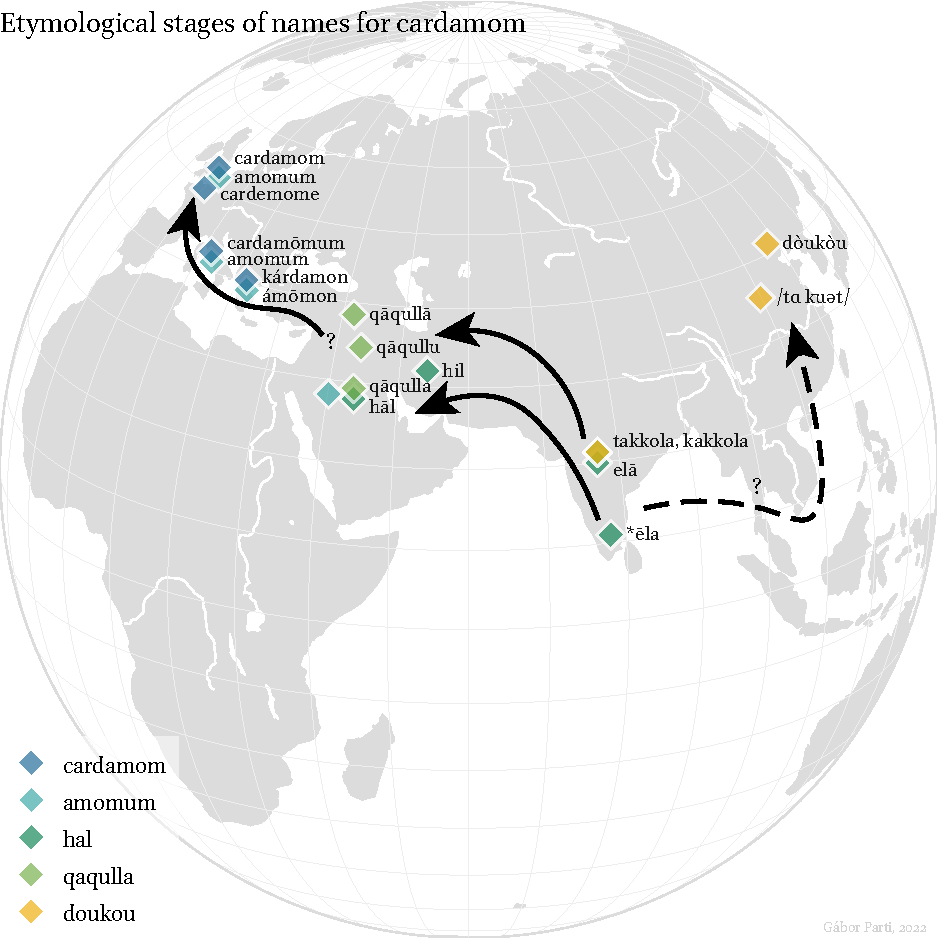
\includegraphics[width=\textwidth]{imgs/plots/diffusion_cardamom_edited.pdf}
    \caption[Diffusion of names for cardamom, and their etymological stages.]{Diffusion of names for cardamom, and their etymological stages in English, Arabic, and Chinese.}
    \label{fig:diffusion_cardamom}
\end{figure}







% MW:
% Latin cardamomum, from Greek kardamōmon, blend of kardamon garden peppergrass \& amōmon, an Indian spice plant

